\chapter{General concepts}
This chapter discusses the main concepts used in a \Vaango simulation.
These concepts are independent of the type of problem being considered
and are core to the computational framework.  Special treatment is needed
for components such as \Textsfc{MPM} or \Textsfc{Peridynamics}.

\section{Scheduler}

The Scheduler in \Vaango is responsible for determining the order of
tasks and ensuring that the correct inter-processor data is made
available when necessary. Each software component passes a set of
tasks to the scheduler. Each task is responsible for computing some
subset of variables, and may require previously computed variables,
possibly from different processors. The scheduler will then compile
this task information into a task graph, and the task graph will
contain a sorted order of tasks, along with any information necessary
to perform inter-process communication via MPI or threading. Then, when the
scheduler is executed, the tasks will execute in the pre-determined
order.

\subsection{needRecompile()}

%% Not sure where this information really should go, but wanted to
%% save it for posterity...

Each component has a \Textsfc{needRecompile()} function that is called once per
timestep.  If, for whatever reason, a Component determines that the
list of tasks it had previously scheduled is no longer valid, then the
Component must return `true' when its \Textsfc{needRecompile()} function is
called.  This will cause the scheduler to rebuild the task graph (by
asking each component to re-specify tasks).  Note, rebuilding the
taskgraph is a relatively expensive operation, so only should be done
if necessary.

\section{Tasks}

A task contains two essential components: a pointer to a function
that performs the actual computations, and the data inputs and
outputs, i.e. the data dependencies required by the function.  When a
task requests a previously computed variable from the data warehouse,
the number of ghost cells are also specified.  The Unitah framework
uses the ghost cell information to excecute inter-process
communication to retrieve the necessary ghost cell data.

An example of a task description is presented showing the essential
features that are commonly used by the application developer when
implementing an algorithm within the \Vaango framework.  The task
component is assigned a name and in this particular example, it is
called \Textsfc{taskexample} and a function pointer,
\Textsfc{\&Example::taskexample}.  Following the instantiation of the
task itself, the dependency information is assigned to the tasks.  In
the following example, the task requires data from the previous
timestep (\Textsfc{Task::OldDW}) associated with the name
variable1\_label and requires one ghost node
(\Textsfc{Ghost::AroundNodes,1}) level of information which will be
retrieved from another processor via MPI.  In addition, the task will
compute two new pieces of data each associated with different
variables, i.e. \Textsfc{variable1\_label}, and
\Textsfc{variable2\_label}.  Finally, the task is added to the scheduler
component with specifications about what patches and materials are
associated with the actual computation.

\begin{lstlisting}[language=Cpp]
  Task* task = scinew Task("Example::taskexample",this, &Example::taskexample);
  task->requires(Task::OldDW, variable1_label, Ghost::AroundNodes, 1);
  task->computes(variable1_label);
  task->computes(variable2_label);
  sched->addTask(task, level->eachPatch(), sharedState_->allMaterials());
\end{lstlisting}

For more complex problems involving multiple materials and
multi-physics calculations, a subset of the materials may only be used
in the calculation of particular tasks.  The \Vaango framework allows
for the independent scheduling and computation of multi-material
within a multi-physics calculation.

\section{Simulation Component Class Description}

Each \Vaango component can be described as a C++ class that is derived
from two other classes: \Textbfc{UintahParallelComponent} and a
\Textbfc{SimulationInterface}. The new derived class must provide the
following virtual methods: \Textsfc{problemSetup},
\Textsfc{scheduleInitialize}, \Textsfc{scheduleComputeStableTimestep},
and \Textsfc{scheduleTimeAdvance}.  Here is an example of the typical
*.h file that needs to be created for a new component.

\begin{lstlisting}[language=Cpp]
  class Example : public UintahParallelComponent, public SimulationInterface {
    public:

      virtual void problemSetup(const ProblemSpecP& params, const ProblemSpecP& restart_prob_spec, GridP& grid, SimulationStateP&);

      virtual void scheduleInitialize(const LevelP& level,SchedulerP& sched);
    
      virtual void scheduleComputeStableTimestep(const LevelP& level, SchedulerP&);
    
      virtual void scheduleTimeAdvance(const LevelP& level, SchedulerP&);

    private:
      Example(const ProcessorGroup* myworld);
      virtual ~Example();


      void initialize(const ProcessorGroup*, const PatchSubset* patches, const MaterialSubset* matls, DataWarehouse* old_dw, DataWarehouse* new_dw);
    
    
      void computeStableTimestep(const ProcessorGroup*, const PatchSubset* patches, const MaterialSubset* matls, DataWarehouse* old_dw, DataWarehouse* new_dw);
    
      void timeAdvance(const ProcessorGroup*, const PatchSubset* patches, const MaterialSubset* matls, DataWarehouse* old_dw, DataWarehouse* new_dw);
  }
\end{lstlisting}

Each new component inherits from the classes
\Textbfc{UintahParallelComponent} and \Textbfc{SimulationInterface}.
The component overrides default implementations of various methods.
The above methods are the essential functions that a new component
must implement.  Additional methods to do AMR will be described as
more complex examples are presented.

The roles of each of the scheduling methods are described below.  Each
scheduling method, i.e. \Textsfc{scheduleInitialize},
\Textsfc{scheduleComputeStableTimestep}, and
\Textsfc{scheduleTimeAdvance} describe

\subsection{ProblemSetup}

The purpose of this method is to read a problem specification which
requires a minimum of information about the grid used, time
information, i.e. time step size, length of time for simulation, etc,
and where and what data is actually saved.  Depending on the problem
that is solved, the input file can be rather complex, and this method
would evolve to establish any and all parameters needed to initially
setup the problem.

\subsection{ScheduleInitialize}

The purpose of this method is to initialize the grid data with values
read in from the problemSetup and to define what variables are
actually computed in the TimeAdvance stage of the simulation.  A task
is defined which references a function pointer called
\Textsfc{initialize}.

\subsection{ScheduleComputeStableTimestep}

The purpose of this method is to compute the next timestep in the
simulation.  A task is defined which references a function pointer
called \Textsfc{computeStableTimestep}.

\subsection{ScheduleTimeAdvance}

The purpose of this method is to schedule the actual algorithmic
implementation.  For simple algorithms, there is only one task defined
with a minimal set of data dependencies specified.  However, for more
complicated algorithms, the best way to schedule the algorithm is to
break it down into individual tasks.  Each task of the algorithm will
have its own data dependencies and function pointers that reference
individual computational methods.

\section{Data Storage Concepts}

During the course of the simulation, data is computed and stored in a
data structure called the DataWarehouse.  The DataWarehouse is an abstraction
for storage, retrieval, and access of \Vaango simulation data. The Data warehouse 
presents a localized view of the global data distribution.  

\subsection{Data Archiver}

The Data Archiver is a component of the framework that allows for reading, saving, 
and accessing simulation data. 
It presents a global shared memory abstraction to the simulation data. The component 
developer does not have 
to worry about retrieving data that has been produced on a remote processor or 
sending data from a local processor 
to another processor for use. The framework takes care of these tasks implicitly 
for the component. 

\subsection{Two Data Warehouses}
During each time step (assuming a single level problem), there are two data 
warehouses associated with the simulations. The \Textttc{new\_dw} and the 
\Textttc{old\_dw} (as they are commonly referred to in the code). The 
\Textttc{old\_dw} contains data that was generated in the previous timestep, 
and may not be modified. Data that is generated during the current timestep will 
be placed in the \Textttc{new\_dw}. At the end of a timestep, the current 
\Textttc{old\_dw} is deleted, and then replaced with the 
current \Textttc{new\_dw}. Then a new (empty) \Textttc{new\_dw} is created.

At the end of a time step, some data is automatically transferred from the 
current time step's \Textttc{new\_dw} into the next 
time step's \Textttc{old\_dw}. 

\subsection{Storing and Retrieving Variables}
In order to store data to the data warehouse, or to retrieve data, several 
things are required. First, the task (which procedure wishes access to the 
data) must have registered this information with the Scheduler during task 
creation time. Then, inside of the task, the following call is used to pull 
the data from the data warehouse: 

\begin{lstlisting}[language=Cpp]
  SFCXVariable<double> uVelocity;
  new_dw->get( uVelocity, d_lab->d_uVelocitySPBCLabel, matlIndex, patch, Ghost::AroundFaces, Arches::ONEGHOSTCELL ); 
\end{lstlisting}

Similarly, to put data into the data warehouse, use this call: 
\begin{lstlisting}[language=Cpp]
  PerPatch<CellInformationP> cellInfoP;
  new_dw->put( cellInfoP, d_lab->d_cellInfoLabel, matlIndex, patch ); 
\end{lstlisting}

\subsection{Variables}
There are three (general) types of variables in \Vaango: Particle, Grid, and Reduction. 
Each type of variable is discussed below. Remember, in order to interact with the 
Data Warehouse, each variable must have a corresponding label. 

\Textsfc{Particle variables} contain information about particles. 

A \Textsfc{grid variable} is a representation of data across (usually) the entire 
computational domain. It can be used to represent 
temperature, volume, velocity, etc. It is implemented using a 3D array. 

A \Textsfc{reduction}, in terms of distributed software (using, for example, MPI) is 
a point in which all (or some defined set of) processors all communicate with 
each other. It usually is an expensive operation (because it requires all 
processors to synchronize with each other and pass data). However, many times 
this operation cannot be avoided. \Vaango provides a "Reduction Variable" to 
facilitate this operation. Common reductions operations include finding the 
min or max of a single number on all processors, or creating the sum of a 
number from every processor, and returning the result to all processors. 

Variables can be stored at several different locations. Variables are defined 
with respect to how they relate to a single cell in the computational 
domain. They may be located on the faces (FC) or nodes (NC) of the cell, 
or in the center (CC) of the cell (see Figure \ref{Fig:DWVariablesCell}). 
\begin{figure}
  \centering
  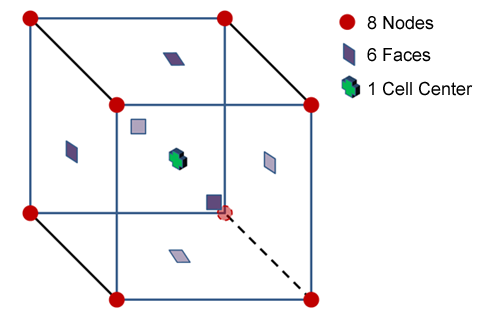
\includegraphics[width=0.5\textwidth]{DWVariablesCell.png}
  \caption{Variable locations with respect to a single cell.}
  \label{Fig:DWVariablesCell}
\end{figure}



\section{Grid data}
Data (Variables) used by the framework are stored on the \Textsfc{Grid}. The Grid is comprised 
of one or more (in the case of AMR) Levels. Each level contains one or more patches; and each 
patch contains a number of cells. The simulation data itself exists in (at) each cell (and 
is stored in a 'variable' which is implemented as a 3D array of the data in each cell across 
the patch).

\subsection{Cells}
Data in (at) each cell can be specified in several ways. Specifically the data can be 
\Textsfc{Node centered} (NC), \Textsfc{Cell centered} (CC), or \Textsfc{Face centered} (FC). 
For CC data, there is one value associated with each cell; for NC data, 4 values; and 
for FC data, 6 values. 

\subsection{Patches}
For calculations to take place on a patch, information from bordering patches is 
required. This information is stored in boundary cells. 

\subsection{Boundary Cells}
\begin{figure}
  \centering
  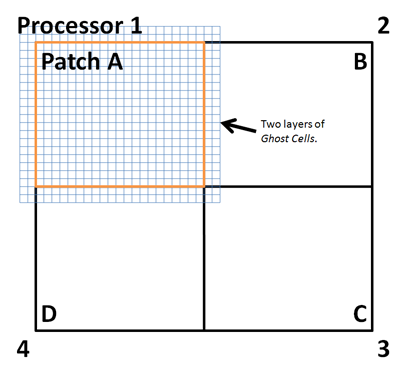
\includegraphics[width=0.5\textwidth]{GhostCells.png}
  \caption{Schematic of ghost cell locations laid out with respect to patches.}
  \label{Fig:GhostCells}
\end{figure}

Boundary cells (Figure \ref{Fig:GhostCells}) represent portions of the computational 
domain outside the boundaries of the data assigned to a given processor. Specifically, 
they are almost always used as boundary cells to a patch that are necessary for 
computation, but are not ``owned'' by the patch that is currently being computed. As 
can be seen in Figure \ref{Fig:GhostCells}, patch A owns all the cells within the 
orange rectangle, but also has two layers of ghost cells. Portions of these cells 
are actually owned by patches B, C, and D. (The data found in these cells is 
automatically transfered (by the framework) from processors 2, 3, and 4 to processor 
1 in order for the cell data to be available for use in computations on patch A.)

Many operations will require a stencil consisting of several cells in order to 
perform calculations at a given cell. However, at the border of a patch, there 
are no cells belonging to that patch that contain the required information - that 
information is ``owned'' by another processor.  In this situation, data that 
belongs to another patch must be accessed. This is the purpose of ghost cells. The 
Data Warehouse takes care of moving the required ghost data from the ``owner'' 
processor to the neighbor processor so that the individual task can assume the 
required data is available. 

In summary, ghost cells exist between patches on the same level.  They are cells 
that are owned by the neighboring patch but are required for computation due to 
the stencil width.

Extra cells exist at the edge of the computational domain and are used for 
boundary conditions.  Extra cells exist on the boundaries of the level where 
no neighboring patches exist. This can either be the edge of a domain or 
on a coarse-fine interface.

\subsection{Indexing grid cells}
\Vaango uses a straightforward indexing scheme. Each cell on a given level is 
uniquely identified by an x,y,z coordinate (stored in an \Textttc{IntVector}).  
An IntVector is a vector of 3 integers that represent an X,Y,Z coordinate.  
See \Textsfc{Core/Grid/Level.cc/h} for more information.  The following pseudo 
code shows how indices across levels are mapped to each other.

\begin{lstlisting}[language=Cpp]
IntVector
Level::mapCellToCoarser(const IntVector& idx) const
{ 
  IntVector ratio = idx/d_refinementRatio;
  
  return ratio;
}

IntVector
Level::mapCellToFiner(const IntVector& idx) const
{
  IntVector r_ratio = grid->getLevel(d_index+1)->d_refinementRatio;
  IntVector fineCell = idx*r_ratio;

  return fineCell;
}
\end{lstlisting}





